\documentclass[tikz,border=2pt]{standalone}

\usepackage{pgfplots}
\pgfplotsset{compat=1.18}

\begin{document}
	
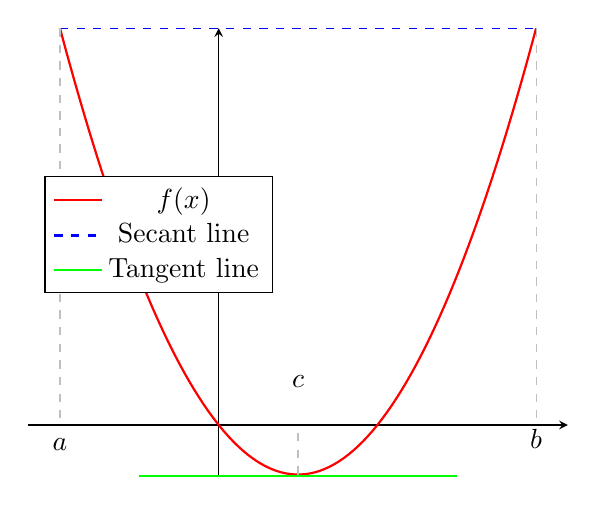
\begin{tikzpicture}
	\begin{axis}[
		axis lines = middle,
		legend pos = north west,
		xtick=\empty, 
		ytick=\empty,
		xmin=-1.2,  % Adjust left margin
		xmax=2.2,   % Adjust right margin
		legend style={at={(0.03,0.67)},anchor=north west},
		]
		
		% Define the function
		\addplot[
		domain=-1:2, 
		samples=100, 
		color=red,
		thick,
		]
		{x^2 - x};
		\addlegendentry{\(f(x)\)}
		
		% Define points a, b, and c
		\def\pointA{-1}
		\def\pointB{2}
		\def\pointC{0.5}
		
		% Add nodes for a, b, and c
		\node[coordinate,label=below:\(a\)] at (axis cs:\pointA,-0.02) {};
		\node[coordinate,label=below:\(b\)] at (axis cs:\pointB,0.03) {};
		\node[coordinate,label=below:\(c\)] at (axis cs:\pointC,0.3) {};
		
		% Draw secant line
		\addplot[dashed, color=blue, thick, domain=-1:2] {2};
		\addlegendentry{Secant line}
		
		% Draw tangent line at c
		\addplot[domain=-0.5:1.5, color=green,thick] {-0.26};
		\addlegendentry{Tangent line}
		
		% Draw dashed lines for a, b, and c
		\addplot[dashed,color=lightgray] coordinates {(\pointA, 2) (\pointA, 0)};
		\addplot[dashed,color=lightgray] coordinates {(\pointB, 2) (\pointB, 0)};
		\addplot[dashed,color=lightgray] coordinates {(\pointC, -1/4) (\pointC, 0)};
	\end{axis}
\end{tikzpicture}
	
\end{document}